\documentclass[10pt,nofootinbib]{revtex4}
\usepackage{amsmath,amssymb,amsfonts,mathrsfs,bm,dsfont}
\usepackage{enumerate}
\usepackage[all]{xy}
\usepackage[normalem]{ulem}	% delete line
\usepackage{graphics,color}
\usepackage{tikz}
	\usetikzlibrary{calc}
	\usetikzlibrary{decorations.markings}
	\usetikzlibrary{arrows}
	\usetikzlibrary{patterns}
\usepackage{pgfplots}


%\usepackage{hyperref}
\usepackage{feynmp} % feymann diagram
\usepackage{extarrows}


\newcommand*\dd{\mathop{}\!\mathrm{d}}
\newcounter{Claim}[section]
\newenvironment{Claim}[1][]{{\par\normalfont\bfseries \underline{Claim~\stepcounter{Claim}\arabic{Claim}.}~#1~~}}{\par}
\newcounter{Proposition}[section]
\newenvironment{Proposition}[1][]{{\par\normalfont\bfseries \underline{Proposition~\stepcounter{Proposition}\arabic{Proposition}.}~#1~~}}{\par}
\newcounter{Note}[section]
\newenvironment{Note}[1][]{{\par\normalfont\bfseries \underline{Note~\stepcounter{Note}\arabic{Note}.}~#1~~}}{\par}
\newcounter{Lemma}[section]
\newenvironment{Lemma}[1][]{{\par\normalfont\bfseries \underline{Lemma~\stepcounter{Lemma}\arabic{Lemma}.}~#1~~}}{\par}
\newcounter{Corollary}[section]
\newenvironment{Corollary}[1][]{{\par\normalfont\bfseries \underline{Corollary~\stepcounter{Corollary}\arabic{Corollary}.}~#1~~}}{\par}
\newenvironment{Proof}{{\par~{\normalfont\bfseries $\vartriangleright$}~~}}{\hfill $\square$\par\hfill\par} %\par
\newcounter{Def}[section]
\newenvironment{Def}[1][]{{\par\normalfont\bfseries \underline{Definition~\stepcounter{Def}\arabic{Def}.}~#1~~}}{\par}

\allowdisplaybreaks[4] %允许 align 跨页编排

\def\Re{\mathop{\mathcal{R}e}}
\def\Im{\mathop{\mathcal{I}m}}
\def\imp{\text{imp}}

\def\arrow{\tikz[scale=0.1,baseline=.1ex]{
	\draw[fill=black,rotate=-90] (-0.7,0)--(0,2)--(0.7,0);}
	}

\def\cross{\tikz[scale=0.1,baseline=.1ex]{
	\draw[thick,rotate=45] (-1,0)--(1,0);
	\draw[thick,rotate=45] (0,-1)--(0,1);}
	}





\begin{document}
\title{Conformal Field Theory and Applications in Condensed Matter Physics}% Force line breaks with \\
%\thanks{This is a reminiscent note for Hubbard-Stratonovich Transformation.}%

\author{Xiaodong Hu}
%\altaffiliation[Also at ]{Boson College}
\email{xiaodong.hu@bc.edu}
\affiliation{Department of Physics, Boston College}

\date{\today}

\begin{abstract}
	This is a research note about applied CFT. For example, we will discuss the single-loop RG equation by OPE and the boundary CFT of bulk FQHE.
\end{abstract}
\maketitle
\tableofcontents
\section{General Conformal Transformation}
	Let us consider a local field theory defined on a $D$-dimensional spacetime with \emph{Euclidean} metric $g_{\mu\mu}\equiv\eta_{\mu\nu}$ and signature $(p,q)$. A general diffeomorphism transforms the metric to 
	\begin{equation*}
		g_{\mu\nu}\mapsto \widetilde{g}_{\mu\nu}(\widetilde{x} )\equiv\dfrac{\partial x_\mu }{\partial \widetilde{x}_\alpha }\dfrac{\partial x_\alpha}{\partial \widetilde{x}_\beta }g_{\alpha\beta}.
	\end{equation*}
	\begin{Def}[(Conformal Group)]
		Conformal group is the subgroup of diffeomorphism group leaving the metric tensor unchcanged up to a scaling factor
		\begin{equation}\label{1.1.1}
			\widetilde{g}_{\mu\nu}(\widetilde{x})=\Omega(x)g_{\mu\nu}(x). 
		\end{equation}
		Clearly Poincar\'{e} group ($\Omega\equiv1$) is the subgroup of confromal group.
	\end{Def}
	\hfill\par
	The full generators of conformal transformation is obtained by solving the allowed infinitesimal transformation $\widetilde{x}_\mu\equiv x_\mu+\varepsilon_\mu+\mathcal{O}(\varepsilon^2) $ such that
	\begin{align*}
		\widetilde{g}_{\mu\nu} &\equiv(\delta^\alpha_\mu+\partial_\mu \varepsilon^\alpha)(\delta^\beta_\nu+\partial_\nu \varepsilon^\beta)g_{\alpha \beta}=g_{\mu\nu}+\partial_\mu \varepsilon^\alpha g_{\alpha\nu}+\partial_\nu \varepsilon^\beta g_{\mu \beta}+\mathcal{O}(\varepsilon^2)\\
		&=g_{\mu\nu}+(\partial_\mu \varepsilon_\nu+\partial_\nu \varepsilon_\mu)+\mathcal{O}(\varepsilon^2)
	\end{align*}
	from the constriant \eqref{1.1.1}
	\begin{equation}\label{1.1.2}
		(\partial_\mu \varepsilon_\nu+\partial_\nu \varepsilon_\mu)=(\Omega(x)-1)g_{\mu\nu}\equiv f(x)g_{\mu\nu}.
	\end{equation}
	Tracing both sides with $g^{\mu\nu}$ 
	\begin{equation*}
		2\partial^\mu \varepsilon_\mu=f(x)D,
	\end{equation*}
	we then can eliminate the newly defined scaling factor $f(x)$ by inserting back to equation \eqref{1.1.2}
	\begin{equation}\label{1.1.3}
		\boxed{(\partial_\mu \varepsilon_\nu+\partial_\nu \varepsilon_\mu)=\dfrac{2}{D}(\partial \cdot \varepsilon)g_{\mu\nu}.}
	\end{equation}
	Since equation \eqref{1.1.3} degenerates for 1d spacetime (so the theory is trivial), we will focus on the case when $D\geq2$.
	\begin{itemize}
		\item For $D=2$, equation \eqref{1.1.3} gives the celebrated \emph{Cauchy-Riemann equation}
		\begin{equation}\label{1.1.4}
			\partial_1 \varepsilon_2\equiv-\partial_2 \varepsilon_1,\quad \partial_1 \varepsilon_1\equiv \partial_2 \varepsilon_2.
		\end{equation}
		\item But for $D>2$, we have to to re-arrange \eqref{1.1.3} into a more explicit form. Applying $\partial^\nu$ with $\partial_\nu$ on \eqref{1.1.3} gives
		\begin{equation}\label{1.1.5}
			\partial_\mu\partial_\nu(\partial \cdot \varepsilon)+\partial^2\partial_\nu\varepsilon_\mu=\dfrac{2}{D}\partial_\mu \partial_\nu(\partial\cdot\varepsilon).
		\end{equation}
		Similarly for the twice derivatives of $\partial_\mu$ and $\partial^\mu$
		\begin{equation}\label{1.1.6}
			\partial^2\partial_\mu\varepsilon_\nu+\partial_\nu\partial_\mu(\partial \cdot \varepsilon)=\dfrac{2}{D}\partial_\nu \partial_\mu(\partial\cdot\varepsilon).
		\end{equation}
		Then by adding up \eqref{1.1.5} and \eqref{1.1.6} and inserting \eqref{1.1.3} to replace $(\partial_\mu \varepsilon_\nu+\partial_\nu \varepsilon_\mu)$, we obtain the simple differential equation of $(\partial\cdot\varepsilon)$
		\begin{equation}\label{1.1.7}
			2\partial_\mu \partial_\nu(\partial\cdot\varepsilon)+\partial^2\left(\dfrac{2}{D}(\partial\cdot \varepsilon)g_{\mu\nu}\right)=\dfrac{4}{D}\partial_\mu \partial_\nu(\partial\cdot\varepsilon)\implies (g_{\mu\nu}\partial^2+(D-2)\partial_\mu \partial_\nu)(\partial\cdot \varepsilon)=0 \implies (D-1)\partial^2(\partial \cdot \varepsilon)=0.
		\end{equation}
	\end{itemize}
	
	\subsection{Conformal Transformation in $D>2$}
		For $D>2$ the constraint \eqref{1.1.7} implies the infinitesimal $\varepsilon_\mu$ to be at most \emph{quadratic} in coordinate
		\begin{equation*}
			\varepsilon_\mu=a_\mu+b_{\mu\nu}x^\nu+c_{\mu\nu\rho}x^\nu x^\rho
		\end{equation*}
		with the symmetric $c_{\mu\nu\rho}\equiv c_{\mu\rho\nu}$.\par
		\begin{enumerate}[1)]
			\item Clearly $\varepsilon_\mu=a_\mu$ represents the (infinitesimal) \textbf{space-time translation} $x'_\mu\mapsto x_\mu+a_\mu$ as ususal.
			\item By inserting $\varepsilon_\mu=b_{\mu\nu}x^\nu$ back into \eqref{1.1.3} we have
				\begin{equation*}
					b_{\mu\nu}+b_{\nu\mu}=\dfrac{2}{D}(b_{\alpha\beta} \partial^\alpha x^\beta) g_{\mu\nu}=\dfrac{2}{D}b_\alpha^{~\alpha}g_{\mu\nu}.
				\end{equation*}
				Separating $b_{\mu\nu}$ into symmetric part $b^s_{\mu\nu}\equiv b^s_{\mu\nu}$ and anti-symmetric part $b^a_{\mu\nu}\equiv-b^a_{\mu\nu}$, then the anti-symmetric part represents the familiar (infinitesimal) \textbf{space-time rotation} $b^a_{\mu\nu}\equiv\omega_{\mu\nu}$, while the symmetric part $b^s_{\mu\nu}=\dfrac{1}{D}(b^s)_\alpha^{~\alpha}g_{\mu\nu}$ represents the (infinitesimal) \textbf{space-time dilation} since
				\begin{equation*}
					x'_\mu=x_\mu+(b^s)_{\mu\nu}x^\nu=\left(1+\dfrac{1}{D}(b^s)_\alpha^{~\alpha}\right)x_\mu\equiv\lambda x_\mu.
				\end{equation*}
			\item By inserting $\varepsilon_\mu=c_{\mu \alpha\beta}x^\alpha x^\beta$ back into \eqref{1.1.3} we have
				\begin{equation*}
					c_{\mu\nu\beta}x^\beta+c_{\nu\mu\beta}x^\beta=\dfrac{2}{D}c^\alpha_{~\alpha\beta}x^\beta g_{\mu\nu}.
				\end{equation*}
				To express $c_{\mu\nu\beta}$ explicitly, we have to cycle all the indices, summing and subtracting them with symmetric condition on the latter two indices of $c_{\mu\nu\beta}$, which yields the \textbf{special conformation transformation} (SCT)
				\begin{equation*}
					c_{\mu\nu\beta}=\dfrac{1}{D}(c^\alpha_{~\alpha\beta}g_{\mu\nu}+c^\alpha_{~\alpha\nu}g_{\mu\beta}-c^\alpha_{~\alpha\mu}g_{\nu\beta})\equiv b_\beta g_{\mu\nu}+b_\nu g_{\mu\beta}-b_\mu g_{\nu\beta}
				\end{equation*}
				with $b_\beta\equiv c^\alpha_{~\alpha\beta}/D$. So the coordinate transforms (infinitesimally) as
				\begin{equation*}
					x'_\mu=x_\mu+2(b\cdot x)x_\mu-b_\mu x^2.
				\end{equation*}
		\end{enumerate}
		\hfill\par
		The full four generators for these \emph{infinitesimal} conformal transformations can be directly read out as in table \ref{tab:1} because on the one side, the infinitesimal transformation parameterized by $\omega_a$ can be written as $x'_\mu(x)\simeq x_\mu+\dfrac{\delta x_\mu}{\delta \omega_a}\omega_a=\left(1+\dfrac{\delta x^\nu}{\delta \omega_a}\omega_a\partial_\nu\right)x_\mu $, on the other side by definition of the generator $x'_\mu(x)\equiv e^{iG^a\omega_a}x_\mu\simeq(1+iG^a\omega_a)x_\mu$.
		\begin{table}
			\begin{tabular}{p{2cm}p{12cm}}
				\hline\\[-1em]
				Translation&$P^\alpha=-i\dfrac{\delta}{\delta a_\alpha}(x_\mu+a_\mu)\partial^\mu=-i \partial^\alpha$\\[0.6em]
				Dilation&$D=-i\dfrac{\delta}{\delta\lambda}\lambda x_\mu \partial^\mu=-ix^\mu \partial_\mu$\\[0.6em]
				Rotation&$L^{\alpha \beta}=-i\dfrac{\delta}{\delta \omega_{\alpha \beta}}(x_\mu+\omega_{\mu\nu}x^\nu) \partial^\mu=-i(\delta_{\alpha\mu}\delta_{\beta\nu}-\delta_{\alpha\nu}\delta_{\beta\mu})x^\nu \partial^\mu=i(x^\alpha \partial^\beta-x^\beta \partial^\alpha)$\\[0.6em]
				SCT&$K^\alpha=-i\dfrac{\delta}{\delta b_\alpha}(x_\mu+2(b\cdot x)x_\mu-b_\mu x^2)\partial^\mu=-i(2 x^\alpha (x\cdot \partial )-x^2 \partial^\alpha)$\\[0.8em]
				\hline
			\end{tabular}
			\caption{Corresponding four generators of the infinitesimal conformal transformations.}
			\label{tab:1}
		\end{table}
		After straight-forward but tedious calculations, we can write down the full conformal algebra as following:
		\begin{equation}\label{1.1.8}
		\begin{split}
			[D,D]&=0,\quad[D,P_\mu]=iP_\mu,\quad [D,K_\mu]=-iK_\mu, \quad [D,L_{\mu\nu}]=0,\\
			[P_\mu,P_\nu]&=0,\quad [K_\mu,K_\nu]=0,\quad[K_\mu,P_\nu]=2i(g_{\mu\nu}D-L_{\mu\nu}),\\
			[L_{\mu\nu},L_{\rho\sigma}]&=-i(L_{\mu\rho}g_{\nu\sigma}-L_{\mu\sigma}g_{\nu\rho}-L_{\nu\rho}g_{\mu\sigma}+L_{\nu\sigma}g_{\mu\rho}),\\
			[L_{\mu\nu},P_\rho]&=-i(g_{\mu\rho}P_\nu-g_{\nu\rho}P_\mu),\quad[L_{\mu\nu},K_\rho]=-i(g_{\mu\rho}K_\nu-g_{\nu\rho}K_\mu)
		\end{split}
		\end{equation}

		The four \emph{finite} conformal transformations (namely, the flow) can also be obtained by finding out the integral curve of these generators
		\begin{equation*}
			\dot{x}^\mu=iG^a\omega_a x^\mu.
		\end{equation*}
		Let us take the treaky SCT as an example. The nonlinear ODE
		\begin{equation*}
			\dot{x}^\mu=2(b\cdot x)x_\mu-b_\mu x^2
		\end{equation*}
		is solved by a certain change of variable $I:x^\mu\mapsto y^\mu\equiv x^\mu/x^2$ such that
		\begin{equation}\label{1.1.9}
			\dfrac{x^\mu(t)}{x^2(t)}=\dfrac{x^\mu(0)}{x^2(0)}-tb,\quad\text{or}\quad x^\mu(t)=\dfrac{x^\mu-tb^\mu x^2}{1-2tb\cdot x+(tb)^2 x^2}.
		\end{equation}
		The above change of variable is nothing but the inversion transformation satisfying $I^2\equiv\mathds{1}$. So finite SCT \eqref{1.1.8} can be understood as the inversion with translation and inversion again. The full results are listed as in table \ref{tab:2}.
		\begin{table}
			\begin{tabular}{p{2cm}p{12cm}}
				\hline\\[-1em]
				Translation&$x'_\mu= x_\mu+a_\mu$\\[0.6em]
				Dilation&$x'_\mu= x_\mu+\dfrac{2}{D}(b^s)^\alpha_{~\alpha} g_{\mu\nu}x^\nu\equiv\lambda x_\mu$\\[0.6em]
				Rotation&$x'_\mu= x_\mu+\omega_{\mu\nu}x^\nu$\\[0.6em]
				SCT&$x'_\mu= x_\mu+(b_\beta g_{\mu\nu}+b_\nu g_{\mu\beta}-b_\mu g_{\nu\beta})x^\nu x^\beta\equiv x_\mu+2(b\cdot x)x_\mu-b_\mu x^2$\\[0.6em]
				\hline
			\end{tabular}
			\caption{Four finite conformal transformations.}
			\label{tab:2}
		\end{table}
		
	\subsection{Conformal Transformation in $D=2$}
		For $D=2$, the constraint equation for infinitesimal conformal transformation reduces to beautiful \emph{Cauchy-Riemann equation} \eqref{1.1.4} appearing in complex analysis. So it is natural to introduce the complex variable $z\equiv x_1+ix_2$ and $\bar z\equiv x_1-i x_2$ with the assignment (such that $\partial z=\bar\partial\bar z=1$)
		\begin{equation*}
			\partial\equiv\partial_z=\dfrac{1}{2}(\partial_1-i \partial_2),\quad \bar\partial\equiv\partial_{\bar z}=\dfrac{1}{2}(\partial_1+i \partial_2)
		\end{equation*}
		and also the complex function $\varepsilon(z,\bar z)\equiv(\varepsilon_1+i \varepsilon_2)$, $\bar \varepsilon(z,\bar z)=(\varepsilon_1-i \varepsilon_2)$, to decouple the Cauchy-Riemann equation into \emph{holomorphic} and \emph{anti-holomorphic} modes (or \emph{left-movers} and \emph{right-movers})
		\begin{align*}\label{1.2.1}
			\bar \partial \varepsilon&=0\implies \varepsilon(z,\bar z)=\varepsilon(z),\\
			\partial\bar \varepsilon&=0\implies\bar\varepsilon(z,\bar z)=\bar\varepsilon(\bar z).
		\end{align*}
		Thus two dimensional conformal transformation coincides with the analytic coordinate transformation
		\begin{equation*}
			z\mapsto f(z),\quad \bar z\mapsto\bar f(\bar z).
		\end{equation*}
		\indent Unlike the four kinds of conformal transformation in $D>2$, here by the analyticity of $\varepsilon(z)$ and $\bar\varepsilon(\bar z)$, we can always expand them into Laurent series\footnote{We write the exponent as $n+1$ instead of $n$ just for a convention regarding the components that are well-defined locally. This will not do harm to the structure of Witt Algebra.}
		\begin{equation*}
			\varepsilon(z)=\sum_{n=-\infty}^\infty \alpha_n z^{n+1},\quad \bar\varepsilon(\bar z)=\sum_{m=-\infty}^\infty \beta_m \bar{z}^{m+1}
		\end{equation*}
		with \emph{infinite} number of infinitesimal generators
		\begin{equation}\label{1.2.2}
			\ell_n\equiv-i\dfrac{\delta \varepsilon_n}{\delta \alpha_n}\partial_z=-iz^{n+1}\partial_z,\quad\bar\ell_m\equiv-i\dfrac{\delta\bar\varepsilon_m}{\delta \beta_m}\partial_{\bar z}=-i\bar z^{n+1}\partial_{\bar z}.
		\end{equation}
		They can be easily shown to satisfy the \emph{Witt algebra} $\mathcal{W}$
		\begin{equation}\label{1.2.3}
			[\ell_m,\ell_n]=(m-n)\ell_{m+n},\quad[\bar\ell_m,\bar\ell_n]=(m-n)\ell_n,\quad[\ell_m,\bar\ell_n]=0,
		\end{equation}
		which is clearly the direct sum of two independent subalgebras $\mathcal{W}=\mathcal{A}\bigoplus\bar{\mathcal{A}}$. So let us narrow our discusion to one branch of it.\par
		\begin{Claim}
			\textbf{{\color{red} Although the dimension of $\mathcal{A}$ is infinite, not all the generators are \emph{globally} well defined.}}
		\end{Claim}
		\begin{Proof}
			To reveal this, we can analytically continue the original domain of arbitrary analytic functions
			\begin{equation*}
				\mathop{\mathrm{Dom}}(f)=\{(z,\bar z)\}=\{(x_1,x_2)\}=\mathbb{R}^2
			\end{equation*}
			to $\mathbb{C}^2$ with the ``physical constraint'' $\bar z\equiv z^*$. Then the domain of each branch of conformal transformation, or equivalently analytic coordinate transformation, is now extended form $\mathbb{R}$ to $S^2=\mathbb{C}\bigcup\infty$. All holomorphic conformal transformations are generated from the (tagent) vector field
			\begin{equation*}
				X\equiv X^n \partial_n=\sum_n \alpha_n\ell_n\equiv\sum_n(-i)\alpha_n z^{n+1}\dfrac{\partial }{\partial z^n}.
			\end{equation*}
			Clearly the non-singularity of $X$ as $z\rightarrow0$ demands $n\geq-1$. But to impose the non-singularity of $X$ as $z\rightarrow\infty$, we have to change the variable $z\mapsto1/w$ because the tangent field is only defined in the neighbor of the origin. Then the tagent vector field becomes
			\begin{equation*}
				\widetilde{X}\equiv\widetilde{X}^n\widetilde{\partial}_n=\sum_n\dfrac{\partial w}{\partial z} X^n\dfrac{\partial }{\partial w^n}=\sum_n(-w^2)(-i)\alpha_n\left(\dfrac{1}{w}\right)^{n+1}\dfrac{\partial }{\partial w^n}=\sum_n \alpha_n\left(\dfrac{i}{w}\right)^{n-1}\dfrac{\partial }{\partial w^n}.
			\end{equation*}
			This time the non-singularity of $\widetilde{X}$ as $w\rightarrow\infty$ requires $n\leq1$. Plus the similar argument from another branch, we conclude that \textbf{\color{red}only the conformal transformations generated by $\{\ell_{-1},\ell_0,\ell_1\}\bigcup\{\bar\ell_{-1},\bar\ell_0,\bar\ell_1\}$ are globally well-defined}. 
		\end{Proof}
		



\section{Energy Momentum Tensor}

\section{Radial Quantization}
	\subsection{Virasora Algebra}

\section{Trace Anomaly}

\section{Categorization and Classification of Topological Phases}

\section{Modular Invariance, Moduli Space, and FQHE}

\section{Relation to Entanglement Entropy}

\section{Appendix}
	\subsection{Infinitesimal Symmetric Transformation}
		Geometrically, a classical tensor field $\bm{\Phi}(x)$ is an element of tensor bundle. Positive transformation on the base space-time manifold\footnote{Here without loss of generality we take this transformation to be a mapping between two distinct manifolds. This way of looking is called \emph{positive}. In constrast if one takes such transformation as just a coordinate transformation between two patches of the same manifold, then we call such viewpoint \emph{negative}.} $f:M\rightarrow N, \bm{x}\mapsto \bm{x'}$ will be lifted to the fibers as well
		\begin{equation}\label{A.1.1}
			\bm{\Phi'}(\bm{x'})\equiv \mathscr{F}(\Phi(\bm{x})),
		\end{equation}
		or more clearly in the commutative diagram FIG. \ref{fig: transformation}.\par
		\begin{figure}[!htp]
			\centering
			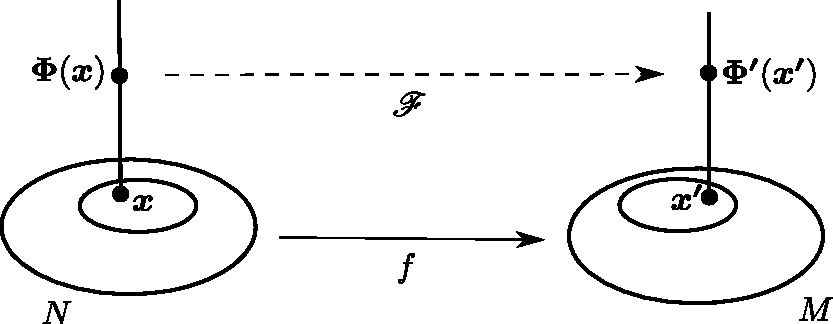
\includegraphics[scale=0.8]{transformation.pdf}
			\caption{{\bf General Transformation}}
			\label{fig: transformation}
		\end{figure}
		For infinitesimal transformation parameterized by some vector $\{\omega_a\}$
		\begin{equation*}
			x'^\mu=x^\mu+\dfrac{\delta x^\mu}{\delta\omega_a}\omega_a+\mathcal{O}(\omega^2),
		\end{equation*}
		identity \eqref{A.1.1} tells
		\begin{equation}\label{A.1.2}
			\bm{\Phi'}(\bm{x'})=\mathscr{F}(\bm{\Phi}(\bm{x}))=\bm{\Phi}(\bm{x})+\dfrac{\delta\mathscr{F}}{\delta\omega_a}\omega_a+\mathcal{O}(\omega^2)
		\end{equation}
		
	\subsection{Noether Theorem and Energy-momentum Tensor}
\bibliography{hxd}
\bibliographystyle{apsrev} % apsrev is format for PRL of APS
\end{document}